% ======================================================================
% TRB Annual Meeting Manuscript
% Converted from the Accident Analysis & Prevention version
% ======================================================================

\documentclass[numbered]{trbunofficial}
\usepackage{float}
% Additional packages required by the manuscript
\usepackage{booktabs}
\usepackage{array}
\usepackage{multirow}
\usepackage{colortbl}
\usepackage{rotating}
\usepackage{xcolor}
\usepackage{subcaption}
\captionsetup[figure]{font=bf,labelsep=space}
\captionsetup[table]{font=bf,labelsep=space}
\captionsetup[subfigure]{font=normalfont,labelsep=space}
\usepackage{microtype}
\usepackage{pgfplots}
\pgfplotsset{compat=1.18}
\usepackage{tikz}
\usetikzlibrary{matrix,positioning,arrows.meta,fit,backgrounds,shapes,calc}

% Colors used in analytical workflow and model-comparison figures
\definecolor{ebike}{RGB}{52, 120, 196}
\definecolor{escooter}{RGB}{70, 160, 70}
\definecolor{bicyclist}{RGB}{220, 150, 50}
\definecolor{other}{RGB}{180, 60, 60}
\definecolor{headerblue}{RGB}{40, 80, 150}
\definecolor{flowblue}{RGB}{210, 228, 252}
\definecolor{flowgreen}{RGB}{208, 240, 208}
\definecolor{flowyellow}{RGB}{255, 248, 210}
\definecolor{floworange}{RGB}{255, 228, 196}

\begin{document}

% ---------- Title Page ----------
\title{Comparative Crash Analysis of E-Bikes, E-Scooters, and Conventional Bicycles Using LLM-Classified Florida Crash Narratives}

\TRBauthor{Rithika Mathew}{Department of Computer and Information Science and Engineering, University of Florida}{rmathew1@ufl.edu}[Gainesville, FL 32611, USA]
\TRBauthor{Yiheng Qian}{Department of Civil and Coastal Engineering, University of Florida}{yihengqian@ufl.edu}[Gainesville, FL 32611, USA]
\TRBauthor{Xingjing Xu}{Department of Urban and Regional Planning, University of Florida}{axuxinjing@ufl.edu}[Gainesville, FL 32611, USA]
\TRBauthor{Ilir Bejleri}{Department of Urban and Regional Planning, University of Florida}{ilir@ufl.edu}[Gainesville, FL 32611, USA]
\TRBauthor*{Xiang Yan}{Department of Civil and Coastal Engineering, University of Florida}{xiangyan@ufl.edu}[Gainesville, FL 32611, USA]

\AuthorHeaders{Mathew, Qian, Xu, Bejleri, and Yan}

\maketitle

% ---------- Structured Abstract ----------
\section{Abstract}

\noindent\textbf{Objectives:}~The rapid growth in e-scooter and e-bike use in recent years has been accompanied by increasing numbers of crashes involving these modes. Addressing these emerging safety concerns requires a better understanding of the factors contributing to e-scooter and e-bike crashes and how they differ from those associated with conventional bicycles. However, Florida crash reports provide no dedicated fields that distinguish electric bicycles (e-bikes) and electric scooters (e-scooters) from conventional bicycles, leaving device type embedded in officer-authored narratives. This study develops and applies a large language model (LLM) framework to recover these modes and compare their crash characteristics.

\hfill\break%
\noindent\textbf{Methods:}~Five LLMs were benchmarked on 300 manually labeled Signal4 Analytics crash narratives from 2015--2025 using a statute-grounded few-shot prompt based on Florida Statute~\S~316.003. The best-performing model was then applied to 2,787 narratives, and the resulting e-bike, e-scooter, and bicyclist records were compared across demographic, temporal, roadway, severity, and crash-scenario attributes.

\hfill\break%
\noindent\textbf{Findings:}~Qwen2.5-72B and Llama~3.1-70B each achieved 98.67\% accuracy, with Qwen2.5-72B selected for full-corpus classification. The classified records included 700 e-scooter, 416 e-bike, and 473 bicyclist crashes. E-scooter riders were youngest and had the highest hit-and-run share, e-bike crashes occurred more often on higher-speed roads, and bicyclists had the highest fatal-injury share. Motorist failure-to-yield was the dominant matched crash scenario across modes.

\hfill\break%
\noindent\textbf{Novelty:}~The study provides a statute-grounded, training-free LLM approach for extracting legally defined micromobility modes from crash narratives and demonstrates its use for statewide comparative safety analysis.

\hfill\break%
\noindent\textbf{Practical Applications:}~The framework can support retrospective mode-specific analysis until structured crash-report fields are updated. The findings also identify distinct infrastructure, reporting, and enforcement priorities for e-scooters, e-bikes, and conventional bicycles.

\newpage

\section{Introduction}
\label{sec:intro}

% e-bike and e-scooter crashes are rising admist the mobility benefits they deliver. To address this emerging safety issue, we understand the crash characteristics and underlying causes, which may be different from conventional bikes.

% despite prior work that provides some preliminary evidence on this topic, we still lack a comprehensive understanding, especially regarding the geographic and environmental contexts associated with e-bike and e-scooter crashes. Police crash reports are a critical data source for shedding light on these issues, but existing crash records do not distinguish e-bike and e-scooter crashes from humna-powered bicycles.

%crash narratives is a promising data source allowing us to classify micromobility crash types, but relying on human labor to read the free-text field is time-consuming and labor intensive.

% this paper 1) develops a LLM-based framework to classify micromobility crashes; 2) examining data in Florida from 2015-2025 (2026？) to provide novel empirical insights regarding differences in crash characteristics; 3) statistical modeling to identify differences in contributing factors (do this after TRB).


Micromobility, which encompasses e-bikes, e-scooters, and conventional bicycles, has emerged as a central component of urban transportation in the United States. Shared e-scooter programs have been deployed in dozens of Florida cities, and consumer adoption of e-bikes has grown rapidly, driven by falling battery costs and expanding bike infrastructure. While micromobility offers meaningful environmental and congestion benefits, these gains are accompanied by measurable increases in crash risk, particularly for users sharing roadways with motor vehicles \citep{Shah2021, Mwambeleko2022}.

A central limitation is that existing crash databases do not readily distinguish micromobility device types or provide the contextual information needed to compare their users and crash conditions. Florida's Uniform Traffic Crash Report (UTCR) system classifies non-motorists primarily as ``bicyclists'' or ``pedestrians,'' with no dedicated fields for e-bike or e-scooter involvement. Crashes involving electrically powered devices are routinely coded in the same category as human-powered bicycles, producing statistics that conflate meaningfully different user populations, speeds, travel patterns, and risk profiles.

The one place where device-specific information reliably appears is in the free-text crash narrative field, where responding officers describe the crash in their own words. Phrases such as ``riding a Bird scooter,'' ``on a motorized bicycle,'' or ``operating a Rad Power e-bike'' appear in thousands of Florida crash records. If these narratives could be classified at scale, they would form the basis of a far more informative micromobility crash database than any structured field currently provides.

Natural language processing (NLP), and specifically large language models (LLMs), offers a practical path toward automating this extraction. LLMs have demonstrated strong performance on complex text classification tasks when supplied with structured prompts and labeled examples \citep{Brown2020, Wei2022}. However, LLMs have not previously been studied at scale for micromobility crash narrative classification, a task in which statutory definitions establish legally precise class boundaries.

This paper addresses three interconnected objectives: (1) systematically evaluate LLMs for classifying micromobility device types in Florida crash narratives; (2) select the best-performing model and apply it to classify the 2,787 crash narratives from the Signal4 Analytics database; and (3) conduct a comparative empirical analysis of demographic characteristics, temporal patterns, spatial distribution, injury severity, and crash scenarios across the three identified micromobility modes.


Our contributions are twofold: (i) a benchmark of five LLM configurations on a 300-sample ground-truth dataset of Florida crash narratives using a statute-grounded few-shot prompt, which shows that Qwen2.5-72B, an open-source model hosted locally on UF’s HiPerGator supercomputer, achieves 98.67\% accuracy at zero marginal inference cost; and (ii) a classified dataset of 1,589 active-mode crash records that enables the first mode-specific comparative analysis of e-bike, e-scooter, and conventional bicycle crashes in Florida at this geographic scale and produces policy-relevant findings on their distinct crash risk profiles.


%Our contributions are: (i) a benchmark of five LLM configurations on a 300-sample ground-truth dataset of Florida crash narratives, developed with a statute-grounded few-shot prompt; (ii) empirical evidence that Qwen2.5-72B, an open-source model hosted locally on UF's HiPerGator supercomputer, achieves 98.67\% accuracy at zero marginal inference cost; (iii) a classified dataset of 1,589 active-mode crash records enabling the first mode-specific comparative analysis of micromobility crashes in Florida at this geographic scale, whereas prior work relies on manual review of small single-city samples rather than LLM-classified statewide records; and (iv) policy-relevant findings on the distinct crash risk profiles of e-bike riders, e-scooter riders, and conventional bicyclists.

%%============================================================
\section{Related Works}
\label{sec:lit}

\subsection{NLP and LLMs for Crash Narrative Analysis}

Free-text police crash narratives have long been recognized as a richer source of incident context than structured coded fields, yet extracting that information at scale has remained a persistent challenge. Early approaches relied on keyword matching and probabilistic classifiers applied directly to narrative text. \citet{Sayed2021} demonstrated that unigram-bigram NoisyOR classifiers could recover work-zone crashes that human coders had miscategorized in structured databases, tracing a lineage from pre-selected keyword lists through progressively more sophisticated text-mining methods. However, such approaches remain limited when vehicle identity depends on context rather than explicit keywords. For example, ``scooter'' may refer to several vehicle types, while e-scooters may be identified indirectly through brand names, propulsion systems, or structural features. Keyword-based methods may also struggle with negation and narratives involving multiple road users.

Transformer-based models provide stronger contextual representations for addressing these challenges. \citet{Hosseini2022} showed that BERT outperformed Naive Bayes, SVM, Decision Tree, Random Forest, and a single-layer perceptron on police-written wrong-way-driving crash reports, achieving 81.6\% accuracy. \citet{Oliaee2023} extended this approach to more than 750,000 crash narratives and achieved 84\% severity classification accuracy, substantially outperforming bag-of-words and TF-IDF methods. Beyond transportation, \citet{Ioannides2022} applied a deep-learning NLP classifier to 36 million clinical notes to identify e-scooter injuries that were not captured by ICD-10 diagnostic codes, achieving 92\% classification accuracy. NLP methods have also been used to extract safety-relevant signals from unstructured text sources beyond formal crash records \cite{Avetisyan2022}. These findings demonstrate the value of contextual language models for extracting safety information that may be obscured or absent in structured records. 

Despite these advances, fine-tuned BERT-style models generally require substantial task-specific labeled data, which can be difficult to obtain for narrowly defined micromobility categories. General-purpose large language models, including GPT- and LLaMA-family models, offer an alternative by using a small number of labeled examples provided within the prompt rather than requiring gradient-based fine-tuning \citep{Brown2020, Min2022}. Prompting models to generate intermediate rationales may also support tasks that require the application of multiple classification rules \citep{Wei2022}. However, classification based on statutory definitions remains challenging because category boundaries are precise, terminology is often inconsistent, and the same term, such as “bike,” may refer to different vehicle types depending on the narrative context. Models may also generate unsupported evidence or overlook relevant details in complex narratives \citep{Ji2023, Liu2024}. Multi-agent frameworks combining voting, confidence selection, or sequential critique have been proposed to improve reliability
\citep{Liang2023, Chen2023}. Whether these approaches provide measurable benefits over a strong single model for a narrowly defined task with near-ceiling performance remains unclear.

%\citet{Avetisyan2022} applied BERTopic and Twitter-RoBERTa to approximately 14,000 geo-located tweets about micromobility in the US and EU, finding that infrastructure and regulatory concerns dominated negative sentiment in both regions while EU users expressed more positive attitudes toward recreational use. This highlights that NLP methods can extract safety-relevant signals from unstructured text sources beyond formal crash records, further motivating their application to crash narrative data.

%%------------------------------------------------------------
\subsection{Micromobility Crash Characteristics}

A parallel body of crash-safety literature has begun to
characterize the distinct risk profiles of e-bikes,
e-scooters, and conventional bicycles. Initial evidence from
emergency department surveillance \citep{Badeau2019,
Trivedi2020} established that e-scooter injuries concentrate
among young adults, frequently involve head trauma, and occur
predominantly on roadways rather than dedicated
infrastructure. However, hospital records provide limited information on roadway context, contributing factors, and motorist actions.

Other data sources have expanded the evidence on rider demographics, crash timing, injury severity, roadway conditions, and motorist behavior. Police records from Nashville showed that e-scooter riders were younger and more likely to be nonlocal than bicyclists, while e-scooter crashes were concentrated in fewer crash types and frequently involved hit-and-run drivers \citep{Shah2021}. Shared e-bike crash records from China linked greater injury severity to younger riders, nighttime conditions, and higher posted speed limits, with additional differences by rider gender \citep{Zhou2025}. National injury surveillance data documented rapid growth in e-bike and powered-scooter injuries, along with higher motor-vehicle involvement for e-bikes and greater alcohol involvement and lower helmet use among powered-scooter riders \citep{Burford2024}. Studies across multiple cities have also associated e-scooter crashes with weekend and evening travel and recurring motorist failure-to-yield scenarios at intersections \citep{Mwambeleko2022}. Together, these studies identify important mode-specific patterns, but most examine individual modes, limited geographic settings, or injury databases with restricted crash-context information. Large-scale U.S. comparisons that distinguish e-bikes, e-scooters, and bicycles within a common crash-record system remain limited. Conducting such a comparison first requires reliable classification of device type from crash narratives.

\subsection{Data Gaps in Micromobility Crash Reporting}

Despite this growing evidence base, three interrelated data gaps limit the field. First, Florida's structured crash fields do not include dedicated categories that consistently distinguish e-bikes, e-scooters, and conventional bicycles, reflecting a broader national reporting limitation identified by the NTSB \citep{NTSB2022}. Second, police-record studies often rely on manual review of relatively small samples, limiting statistical power and geographic coverage \citep{Shah2021}. Third, despite proof of concept in related NLP applications \citep{Sayed2021,Ioannides2022,Oliaee2023}, validated methods for extracting device-type labels from crash narratives at scale remain limited. As a result, large-scale mode-specific comparative analysis remains difficult without first addressing the classification problem. This study focuses on that task.

%%------------------------------------------------------------

\section{Data}
\label{sec:data}

\subsection{Signal4 Analytics}

This study examined crashes involving micromobility devices that occurred in Florida between 2015 and 2025. Crash data were provided by Signal4 Analytics, an interactive, web-based platform designed to support law enforcement agencies and research institutions in crash mapping, data access, and safety analysis. Signal4 aggregates Uniform Traffic Crash Report (UTCR) data from the Florida Department of Highway Safety and Motor Vehicles (FLHSMV), including structured fields and officer-authored free-text narrative descriptions of crash circumstances. The full Signal4 database contains approximately 96,677 crash records involving non-motorists over the study period.

\subsection{From Police Report to Narrative: Data Pipeline}

Before describing the study area and extraction strategy, it is useful to understand how crash information travels from a responding officer to the dataset used in this study. Figure~\ref{fig:pipeline} illustrates this process.

\begin{figure}
\centering
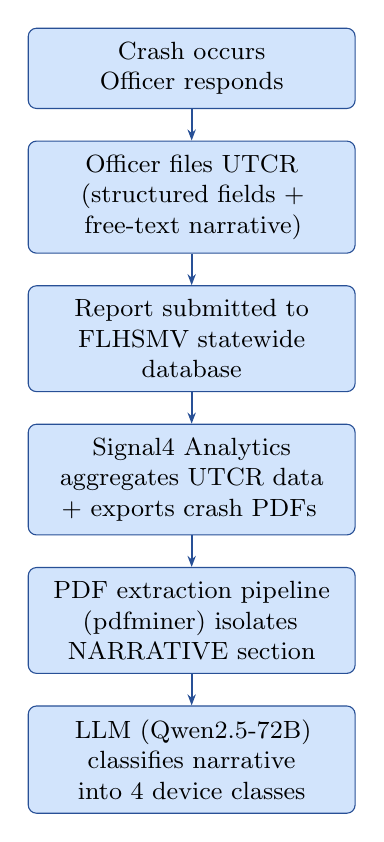
\begin{tikzpicture}[
    stage/.style={rectangle, rounded corners=3pt, draw=headerblue, fill=flowblue,
                  text width=3.8cm, align=center, minimum height=0.9cm,
                  inner sep=5pt, font=\small},
    arrow/.style={-{Stealth[length=4pt]}, thick, headerblue}
]
\node[stage] (crash) {Crash occurs\\Officer responds};
\node[stage, below=0.4cm of crash] (report) {Officer files UTCR\\(structured fields +\\free-text narrative)};
\node[stage, below=0.4cm of report] (hsmv) {Report submitted to\\FLHSMV statewide\\database};
\node[stage, below=0.4cm of hsmv] (signal4) {Signal4 Analytics\\aggregates UTCR data\\+ exports crash PDFs};
\node[stage, below=0.4cm of signal4] (extract) {PDF extraction pipeline\\(pdfminer) isolates\\NARRATIVE section};
\node[stage, below=0.4cm of extract] (llm) {LLM (Qwen2.5-72B)\\classifies narrative\\into 4 device classes};
\draw[arrow] (crash) -- (report);
\draw[arrow] (report) -- (hsmv);
\draw[arrow] (hsmv) -- (signal4);
\draw[arrow] (signal4) -- (extract);
\draw[arrow] (extract) -- (llm);
\end{tikzpicture}
\caption{From crash event to classified record. Structured UTCR fields do not distinguish e-bikes from conventional bicycles; device-type information is recoverable only from the free-text narrative section of the police crash report PDF.}
\label{fig:pipeline}
\end{figure}

When a crash occurs, the responding officer files a Uniform Traffic Crash Report (UTCR) that includes both structured coded fields and a free-text narrative section written in the officer's own words. These reports are submitted to the Florida Department of Highway Safety and Motor Vehicles (FLHSMV) and subsequently aggregated by Signal4 Analytics, which exports individual crash records as PDF files. Because the device-type information critical to this study (e.g., ``Bird scooter,'' ``Rad Power e-bike'') appears only in the narrative section and not in any structured field, a custom extraction pipeline was developed to isolate and retrieve that text.

\subsection{Narrative Extraction Pipeline}

Crash report PDFs exported from Signal4 were processed using a custom Python script on UF's HiPerGator computing cluster. For each report, the script used \texttt{pdfminer.six} rather than \texttt{PyMuPDF (fitz)} to extract the full text. PyMuPDF strips inter-word spaces because of the font encoding used in these Florida UTCR PDFs, producing unreadable run-together text. The extraction procedure then: (1) normalized page-break characters and stripped repeating page-header boilerplate (report number, agency, date blocks) that pdfminer inserts at the top of each page; (2) located the \texttt{NARRATIVE} section using a regex boundary between the \texttt{NARRATIVE} header and the \texttt{REPORTING OFFICER} block; (3) stripped the officer identification block (dashed separator, ID number, rank, agency, date) that precedes the prose in some reports; and (4) applied a prose-detection heuristic to skip any remaining non-prose form-field lines (e.g., property damage fields, owner addresses) that appeared between the section header and the actual narrative text. The resulting narratives were written to a structured Excel file keyed on the HSMV report number for downstream joining with Signal4 tabular tables.

\subsection{Study Area and Data Extraction}

The entire state of Florida served as the study area. Crash reports were extracted from locations reported to have established micromobility systems in some capacity. These locations included municipalities with active shared e-scooter programs (e.g., Tampa, Miami, Orlando, Gainesville, Jacksonville) and communities with documented e-bike activity or dedicated bicycle infrastructure. This targeted extraction strategy was designed to maximize the concentration of relevant micromobility crash records in the analysis corpus while remaining inclusive of the statewide geographic footprint of e-bike and e-scooter use.

From this extraction, 2,787 crash records were identified as potentially involving a micromobility device, based on a combination of non-motorist type codes and keyword pre-screening of narrative text. These records form the corpus classified in the present study.
\begin{table}
\centering
\caption{Signal4 Data Tables Used in Analysis}
\label{tab:datasources}
\begin{tabular}{lp{4.8cm}}
\toprule
\textbf{Table (rows)} & \textbf{Key variables used} \\
\midrule
\texttt{crash\_event} (96,677) & Date and time, county, light condition, weather, intersection flag, crash type, latitude, and longitude \\
\texttt{non\_motorist} (98,815) & Age, sex, injury severity \\
\texttt{vehicle} (98,874) & Posted speed limit, trafficway code \\
\texttt{bicycle\_typing} (40,902) & Crash group description, bicyclist direction \\
\bottomrule
\end{tabular}
\end{table}
\subsection{Data Structure and Linked Tables}

Signal4 provides crash data across several relational tables joined on a unique report number. The tables used in this analysis are summarized in Table~\ref{tab:datasources}. Tables are joined on report number; one record per crash is retained for demographic and road-environment variables. The \texttt{bicycle\_typing\_20} table codes crash scenarios for bicycle-involved crashes but matched only 14\% of active-mode records because e-scooter and e-bike crashes are typically not routed through the bicycle typing system at the time of reporting. This limits crash-scenario analysis to a subset skewed toward conventional bicycle records.



%%============================================================
\section{Methodology}
\label{sec:methods}

\subsection{Overview}

The analysis proceeds in two stages: (1) an LLM classification benchmark to identify the best-performing model, and (2) application of that model to the full narrative corpus, followed by comparative empirical analysis of the resulting mode-specific datasets. Figure~\ref{fig:workflow} presents the complete analytical workflow.

\begin{figure}
\centering
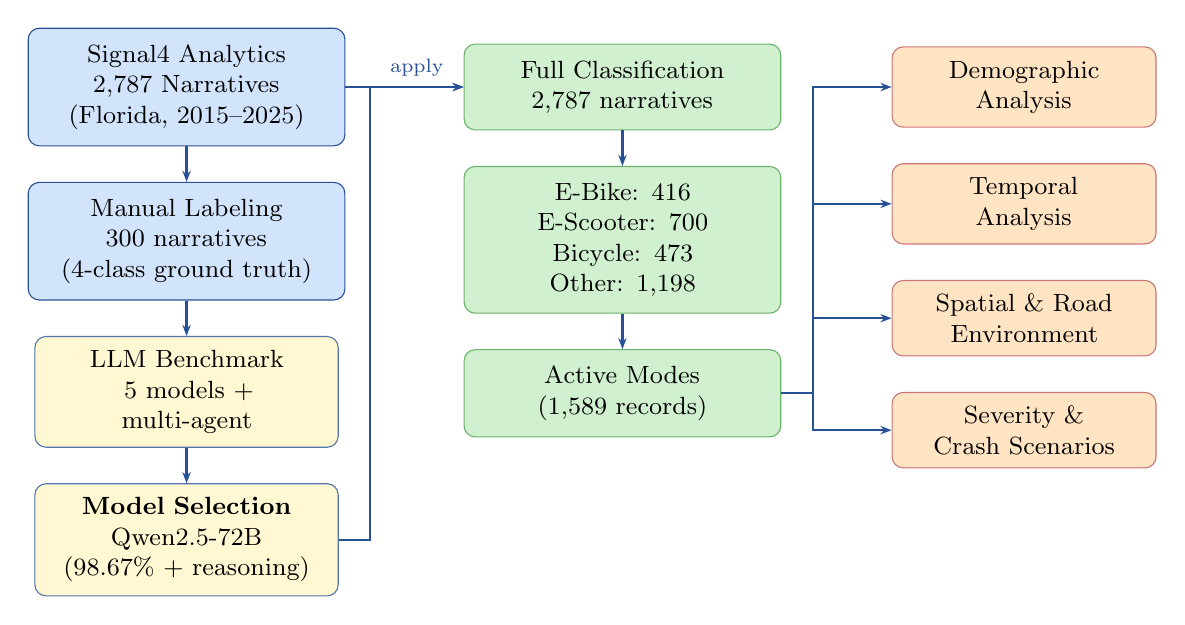
\begin{tikzpicture}[
    box/.style={rectangle, rounded corners=4pt, draw=headerblue, fill=flowblue,
                text width=3.6cm, align=center, minimum height=1.0cm,
                inner sep=6pt, font=\small},
    decision/.style={rectangle, rounded corners=4pt, draw=headerblue!80,
                     fill=flowyellow, text width=3.5cm, align=center,
                     minimum height=1.0cm, inner sep=5pt, font=\small},
    result/.style={rectangle, rounded corners=4pt, draw=escooter!80,
                   fill=flowgreen, text width=3.6cm, align=center,
                   minimum height=1.0cm, inner sep=6pt, font=\small},
    analysis/.style={rectangle, rounded corners=4pt, draw=other!70,
                     fill=floworange, text width=3.0cm, align=center,
                     minimum height=0.9cm, inner sep=5pt, font=\small},
    arrow/.style={-{Stealth[length=4pt]}, thick, headerblue}
]
\node[box] (signal4) {Signal4 Analytics\\2,787 Narratives\\(Florida, 2015--2025)};
\node[box, below=0.45cm of signal4] (manual) {Manual Labeling\\300 narratives\\(4-class ground truth)};
\node[decision, below=0.45cm of manual] (benchmark) {LLM Benchmark\\5 models +\\multi-agent};
\node[decision, below=0.45cm of benchmark] (select) {\textbf{Model Selection}\\Qwen2.5-72B\\(98.67\% + reasoning)};

\node[result, right=1.5cm of signal4] (classify) {Full Classification\\2,787 narratives};
\node[result, below=0.45cm of classify] (classes) {E-Bike: 416\\E-Scooter: 700\\Bicycle: 473\\Other: 1,198};
\node[result, below=0.45cm of classes] (active) {Active Modes\\(1,589 records)};

\node[analysis, right=1.4cm of classify] (demo) {Demographic\\Analysis};
\node[analysis, below=0.45cm of demo] (temporal) {Temporal\\Analysis};
\node[analysis, below=0.45cm of temporal] (spatial) {Spatial \& Road\\Environment};
\node[analysis, below=0.45cm of spatial] (severity) {Severity \&\\Crash Scenarios};

\draw[arrow] (signal4) -- (manual);
\draw[arrow] (manual) -- (benchmark);
\draw[arrow] (benchmark) -- (select);
\draw[arrow] (signal4) -- (classify);
\draw[arrow] (select.east) -- ++(0.4,0) |- (classify.west)
    node[near end, above, font=\scriptsize, text=headerblue]{apply};
\draw[arrow] (classify) -- (classes);
\draw[arrow] (classes) -- (active);
\draw[arrow] (active.east) -- ++(0.4,0) |- (demo.west);
\draw[arrow] (active.east) -- ++(0.4,0) |- (temporal.west);
\draw[arrow] (active.east) -- ++(0.4,0) |- (spatial.west);
\draw[arrow] (active.east) -- ++(0.4,0) |- (severity.west);
\end{tikzpicture}
\caption{Analytical workflow. \textit{Left}: model development pipeline. \textit{Center}: full dataset classification. \textit{Right}: comparative empirical analysis across three active micromobility modes.}
\label{fig:workflow}
\end{figure}

\subsection{Ground-Truth Annotation}

A set of 300 crash narratives was manually labeled to serve as the ground-truth evaluation dataset. Each narrative was reviewed and assigned one of four labels according to Florida Statute~\S~316.003: \textbf{E-bike} (electric bicycle with operable pedals, motor $<$750~W); \textbf{E-scooter} (electric motorized scooter, no pedals); \textbf{Bicyclist} (conventional human-powered bicycle); or \textbf{Other} (mopeds, gas-powered devices, ambiguous narratives, or unconfirmed device type). The labeling process applied a conservative default: when electric power could not be confirmed, narratives were assigned to ``Other'' rather than a specific electric class. Table~\ref{tab:dist} shows the resulting class distribution.

\begin{table}
\centering
\caption{Ground-Truth Class Distribution ($N = 300$)}
\label{tab:dist}
\begin{tabular}{lcc}
\toprule
\textbf{Class} & \textbf{Count} & \textbf{Proportion} \\
\midrule
E-bike     & 52  & 17.3\% \\
E-scooter  & 87  & 29.0\% \\
Bicyclist  & 49  & 16.3\% \\
Other      & 112 & 37.3\% \\
\midrule
\textbf{Total} & \textbf{300} & \textbf{100\%} \\
\bottomrule
\end{tabular}
\end{table}

\subsection{Statute-Grounded Prompt Design and Model Configurations}

All five models were evaluated using a common few-shot prompt structured around four components: (1) verbatim legal definitions from Florida Statute \S~316.003; (2) four-class schema with inclusion, exclusion, and edge-case guidance; (3) a mandatory extraction step requiring the model to enumerate all device terms, power-type evidence, brand signals, and potential conflicts before classifying; and (4) over 40 annotated narrative-label pairs covering the most error-prone patterns.

The prompt was refined through iterative error analysis. Two major error classes were identified: prompt wording errors (ambiguous rules causing inconsistent application) and rule-compliance failures (models not following clear rules). Key refinements included explicit exclusion of infrastructure terms (e.g., ``bicycle lane'') from device extraction, clarification of the human-power override rule, and a bolded warning against stopping at the first device mentioned in a narrative.

Locally hosted models (Qwen2.5-72B, Llama~3.1-70B, DeepSeek-R1-14B) were run on NVIDIA B200 GPU nodes (183~GB VRAM) on the University of Florida's HiPerGator supercomputer at full \texttt{fp16} precision. Commercial models (Claude~3.7~Sonnet, GPT-4o-mini) were accessed via the UF Navigator AI API. All models used greedy decoding (temperature = 0) and produced structured JSON output containing a classification label, confidence score, and reasoning chain.

Three multi-agent architectures were also evaluated using Llama and Qwen as constituent agents: a Dual-Agent Confidence Selector (DACS), which runs both models independently on each narrative and accepts whichever agent's label carries the higher reported confidence score; a Structured Chain-of-Thought (SCoT) pipeline that separates extraction and classification into sequential calls; and a Critique-Guided Reasoning (CGR) pipeline in which Qwen reviews and optionally corrects Llama's output. 

\subsection{Full-Corpus Classification and Cross-Mode Analysis}

The best-performing model identified through the benchmark evaluation was applied to the full corpus of 2,787 crash narratives. Each narrative received a label (E-Bike, E-Scooter, Bicyclist, or Other), a confidence score, and a reasoning chain. The classified dataset was then joined with Signal4 structural tables on report number. The three active modes (E-Bike, E-Scooter, Bicyclist) were compared across five dimensions: demographics (age, sex); temporal patterns (hour, day of week, month, year, and daytime or nighttime conditions); geographic distribution and road environment (county, intersection, speed limit, road type, lighting, weather); injury severity (five-level KABCO scale); and crash scenarios and contributing factors. Narrative keyword analysis was conducted using regex-based term frequency comparison. The ``Other'' class was excluded from all comparative analyses because it is a heterogeneous catch-all category spanning mopeds, gas-powered devices, and narratives where device type could not be confirmed. It does not correspond to a coherent transportation mode and would confound mode-specific comparisons.

%%============================================================
\section{Classification Results and Dataset Overview}
\label{sec:results}

\subsection{Benchmark Performance and Model Selection}
\label{sec:results_llm}


\begin{table}[H]
\centering
\caption{Single-Agent Model Performance ($N = 300$)}
\label{tab:single_agent}
\begin{tabular}{llcc}
\toprule
\textbf{Model} & \textbf{Deploy} & \textbf{Acc.} & \textbf{F1} \\
\midrule
Qwen2.5-72B       & Local  & \textbf{98.67\%} & \textbf{0.99} \\
Llama 3.1-70B     & Local  & \textbf{98.67\%} & \textbf{0.99} \\
Claude 3.7 Sonnet & API    & 98.00\%          & 0.98 \\
GPT-4o-mini       & API    & 93.00\%          & 0.93 \\
DeepSeek-R1-14B   & Local  & 92.95\%          & 0.93 \\
\bottomrule
\end{tabular}
\end{table}

Following the benchmark evaluation, Qwen2.5-72B was selected as the classification model for the full dataset. Table~\ref{tab:single_agent} presents classification accuracy and macro-averaged F1 scores for all single-agent models. Both Qwen2.5-72B and Llama~3.1-70B achieved the highest accuracy (98.67\%), but Qwen was preferred for three reasons. First, Qwen demonstrated more consistent and transparent reasoning chains, explicitly citing device terms and rule numbers in a format that facilitated manual verification. Second, Qwen showed better calibration in difficult cases, particularly in narratives where brand names appeared late in the text, and produced fewer premature classifications. This superior reasoning behavior makes Qwen's output more auditable for a safety-critical classification task. Third, as a locally-hosted open-source model running on HiPerGator, Qwen incurs zero marginal inference cost, unlike commercial APIs such as Claude~3.7~Sonnet or GPT-4o-mini, whose per-token pricing would make full-corpus classification prohibitively expensive at scale.

%Table~\ref{tab:single_agent} presents classification accuracy and macro-averaged F1 scores for all single-agent models. Qwen2.5-72B and Llama~3.1-70B both achieve 98.67\% accuracy, the highest value among the configurations tested. Claude~3.7~Sonnet (98.00\%) is the only commercial model to approach this level. GPT-4o-mini (93.00\%) and DeepSeek-R1-14B (92.95\%) perform substantially lower.




%None of the multi-agent configurations improved over the best single-agent result (Section~\ref{sec:results_llm}); the reasons are analyzed in Section~\ref{sec:discussion}.
Multi-agent architectures did not improve over the best single-agent results. DACS matched Claude~3.7~Sonnet at 98.00\%, while CGR (97.33\%) and SCoT (94.00\%) both underperformed. SCoT's reduced accuracy was driven by hallucination in the extraction step. Models occasionally fabricated electric-power evidence for ambiguous narratives, causing incorrect E-scooter labels. CGR's underperformance is most plausibly explained by anchoring: when Qwen reviewed Llama's initial label, it tended to defer to that label rather than independently reclassify, even when Llama had erred. This behavior limited Qwen's ability to correct Llama's mistakes. These results confirm that added architectural complexity does not translate to improved accuracy on a near-ceiling task.


Application of Qwen2.5-72B to the full narrative corpus yielded 2,787 classified records, of which 1,589 belong to one of the three active micromobility modes (Table~\ref{tab:mode_dist}). E-scooters account for the largest active-mode share (44.1\%). The remaining 1,198 records (43.0\% of the corpus) were assigned to the Other class, which primarily comprises mopeds and gas-powered scooters (identifiable by engine-type references in narratives), device-type-ambiguous reports, and cases where electric power was suspected but not confirmed by the officer's description.

\subsection{Sample Composition and Annual Crash Trends}
\begin{table}
\centering
\caption{Mode Distribution in the Classified Dataset}
\label{tab:mode_dist}
\begin{tabular}{lcc}
\toprule
\textbf{Mode} & \textbf{Crashes} & \textbf{\% Active} \\
\midrule
E-Scooter & 700 & 44.1\% \\
Bicyclist & 473 & 29.8\% \\
E-Bike    & 416 & 26.2\% \\
\midrule
Active total & 1,589 & 100\% \\
Other        & 1,198 & Not applicable  \\
\bottomrule
\end{tabular}
\end{table}

Figure~\ref{fig:annual_trend} shows annual crash counts by mode. Counts for all three modes remained relatively stable through 2020 but began to diverge thereafter. E-scooter crashes increased markedly from 2021 and continued to rise throughout the study period. E-bike crashes followed a broadly similar trajectory, which may reflect the expansion of shared micromobility services and growing ridership in Florida's urban areas. Although e-bike and e-scooter crash counts remained similar through 2024, e-bike crashes increased more sharply in 2025 and clearly exceeded e-scooter crashes. Conventional bicycle crashes showed comparatively modest growth and fell below both powered modes beginning in 2023, indicating that e-bikes and e-scooters had become the two largest contributors to reported micromobility crashes in the classified sample.

%E-bike crashes follow a broadly similar trajectory, with a sustained increase observable from approximately 2021 onward, consistent with the well-documented surge in consumer e-bike adoption during and following the COVID-19 pandemic. 

%, suggesting that the overall rise in micromobility-related incidents is driven primarily by the emergence of electric modes rather than by broader changes in active transportation behavior. It should be noted that the apparent decline across all modes in 2025 is an artifact of incomplete annual reporting rather than a substantive reduction in crash frequency, and should not be interpreted as indicative of an improving safety trend.

\begin{figure}[H]
\centering
\includegraphics[width=0.8\linewidth]{results/qwen_figures/01_overview/01c_annual_trend.png}
\caption{Annual crash counts by mode, 2015--2025.}
\label{fig:annual_trend}
\end{figure}


\section{Mode-specific Crash Analysis}

\subsection{Rider Demographics}



Age and sex distributions are compared in Table~\ref{tab:demographics}. Bicyclists are the oldest group (median 38 years, mean 40.5), with a wide interquartile range consistent with a heterogeneous riding population. E-bike riders are older than expected (median 34, mean 35.3), suggesting this mode is popular among working-age adults. E-scooter users are the youngest (median 26, mean 28.7), concentrated in the 18--37 age range, consistent with shared-mobility demographics in university cities. Males account for 65.6\% of e-bike crashes and 63.6\% of bicycle crashes; e-scooter crashes show a lower male share (51.3\%) and a higher female share (22.9\%). Sex was not recorded for 13--26\% of records per mode, so mode comparisons should be interpreted cautiously.
\begin{table}[H]
\centering
\caption{Demographic Summary by Mode}
\label{tab:demographics}
\begin{tabular}{lccc}
\toprule
 & \textbf{Bicycle} & \textbf{E-Bike} & \textbf{E-Scooter} \\
\midrule
Median age (yr) & 38 & 34 & 26 \\
Mean age (yr)   & 40.5 & 35.3 & 28.7 \\
\% Male         & 63.6 & 65.6 & 51.3 \\
\% Female       & 23.5 & 14.2 & 22.9 \\
\% Sex unknown  & 12.9 & 20.2 & 25.9 \\
\bottomrule
\end{tabular}
\end{table}


\subsection{Time-of-Day, Day-of-Week, and Seasonal Patterns}

All three modes show elevated crash frequencies during the mid-afternoon period from 2 to 6~PM (Figure~\ref{fig:hour_heatmap}), consistent with school dismissal and evening commute activity. E-scooter and e-bike crashes are most concentrated around 4~PM, whereas bicycle crashes are distributed more evenly across the afternoon hours.

%E-bikes show the lowest nighttime crash share ($\approx$13\%), markedly below both e-scooters ($\approx$20\%) and bicycles ($\approx$19\%), supporting a more utilitarian, daylight-hours use profile for this mode.

\begin{figure}[H]
\centering
\includegraphics[width=\linewidth]{results/qwen_figures/03_when/03b_hour_heatmap.png}
\caption{Crash frequency by hour of day and mode.}
\label{fig:hour_heatmap}
\end{figure}

%Figure~\ref{fig:temporal} shows day-of-week and monthly patterns. E-scooter crashes peak on Tuesday (18.6\% of weekly total) and decline on weekends (Saturday 10.9\%, Sunday 9.6\%), consistent with campus- and commute-oriented ridership. Bicycle crashes are distributed more uniformly across the week. E-bike crashes show a Thursday peak (17.5\%), though overall all three modes have similar weekday-to-weekend ratios ($\approx$77--80\% weekday).

Figure~\ref{fig:temporal} shows day-of-week and monthly patterns. Across all three modes, crash frequencies are relatively similar from Monday through Thursday, increase on Friday, decline on Saturday, and reach their lowest levels on Sunday.

Seasonal patterns are broadly similar across the three modes. E-scooter and e-bike crashes peak in April, while bicycle crashes peak in March. Bicycle and e-bike crashes reach their lowest levels in June, whereas e-scooter crashes reach a minimum in July. These declines may reflect reduced ridership during Florida's peak summer heat and, for shared micromobility, the academic off-season. Although the overall seasonal trajectories are comparable, bicycle crashes vary less across months than e-bike and e-scooter crashes.

%Seasonally, bicycle crashes peak in February ($\approx$53) and May ($\approx$52), dropping to a low of 19 in July, which is consistent with reduced ridership during peak summer heat and the academic off-season. E-scooter crashes peak in April ($\approx$77), dip in June--July ($\approx$38--43), then recover in August--October ($\approx$57--60) and reach a secondary peak in December ($\approx$71), potentially reflecting tourist activity and returning university populations. E-bike crashes are relatively elevated in January ($\approx$50) compared to the rest of the year (27--40), with no clear seasonal cycle, suggesting a user base somewhat less sensitive to academic calendars. All three modes show reduced but not equal crash counts in June--July; e-scooter volumes remain roughly twice those of bicycles even at the summer trough.

\begin{figure}
\centering
\begin{subfigure}[b]{0.48\linewidth}
\includegraphics[width=\linewidth]{results/qwen_figures/03_when/03c_day_of_week.png}
\caption{Day-of-week crash counts.}
\end{subfigure}
\hfill
\begin{subfigure}[b]{0.48\linewidth}
\includegraphics[width=\linewidth]{results/qwen_figures/03_when/03d_monthly_pattern.png}
\caption{Monthly crash trends.}
\end{subfigure}
\caption{Temporal distribution of crashes by day of week and month.}
\label{fig:temporal}
\end{figure}

\subsection{Spatial Distribution and Crash Environment}
\begin{figure}[H]
\centering
\includegraphics[width=0.8\linewidth]{results/qwen_figures/04_where/04d_top_counties_stacked.png}
\caption{Top 10 counties by crash count, stacked by mode.}
\label{fig:counties}
\end{figure}
Crashes are concentrated in urbanized areas with active shared-mobility programs (Figure~\ref{fig:counties}), although the modal composition varies across counties. E-scooter crashes account for the largest share in Miami-Dade and Broward counties, where shared scooter services are more prevalent. In contrast, Pinellas and Palm Beach counties have comparatively higher e-bike shares, which may reflect greater e-bike adoption in these areas.



%E-bike crashes occur more often at intersections ($\approx$47\%) than bicycle ($\approx$39\%) or e-scooter crashes ($\approx$40\%). 

All three modes share a median posted speed limit of 30~mph (Figure~\ref{fig:speed}) and show a secondary concentration around 45~mph. However, e-scooter crashes account for a smaller relative share in higher-speed environments, whereas bicycle crashes account for a comparatively larger share. Two-way undivided roads are the dominant roadway type across all three modes (Figure~\ref{fig:roadtype}).

%Bicycles show a bimodal distribution, with a primary concentration at 45~mph and a secondary peak at 25--30~mph. E-scooters ($n = 626$) follow a similar pattern, with a dominant 25--30~mph cluster and a secondary concentration at 45~mph; e-scooter and bicycle crashes both extend to 65~mph road environments. E-bike crashes are capped at 55~mph; while most occur in the 25--35~mph range, approximately 18\% occur at 45~mph speed-limit roads. 

%e-scooters are disproportionately involved in crashes on one-way roads and two-way divided roads with painted medians relative to bicycles and e-bikes. E-scooters have the highest dark-conditions crash share ($\approx$18\% combined dark-lighted and unlit). Clear weather conditions account for $\approx$82--85\% of crashes across all modes, with rain contributing $\approx$4\%.

\begin{figure}
\centering
\begin{subfigure}[b]{0.48\linewidth}
\includegraphics[width=\linewidth]{results/qwen_figures/04_where/04b_speed_limit_violin.png}
\caption{Posted speed limit at crash locations by mode.}
\label{fig:speed}
\end{subfigure}
\hfill
\begin{subfigure}[b]{0.48\linewidth}
\includegraphics[width=\linewidth]{results/qwen_figures/04_where/04c_road_type.png}
\caption{Top Road type at crash locations by mode.}
\label{fig:roadtype}
\end{subfigure}
\caption{Road environment at crash locations.}
\end{figure}

\subsection{Injury Severity Patterns}

Injury severity profiles differ systematically across modes (Table~\ref{tab:severity}). It should be noted that the dataset contains no property-damage-only (PDO) records, as the source data pre-filters to crashes involving at least a possible injury; severity distributions therefore reflect the conditional profile of injury-producing crashes only.

Across the three modes, a clear severity gradient emerges: bicyclists sustain the most severe outcomes, e-bike riders occupy an intermediate position, and e-scooter riders exhibit the lowest rates of serious injury. Specifically, bicycle crashes produce the highest shares of both incapacitating injuries (14.5\%) and fatalities (4.4\%), with the fatal rate exceeding that of e-scooter crashes by more than eightfold (0.5\%). E-bike crashes are characterized by the highest non-incapacitating injury share (50.7\%) and a fatality rate (1.1\%) intermediate between the other two modes, suggesting moderate overall severity. E-scooter crashes, by contrast, concentrate at the lower end of the severity spectrum: the possible-injury share is the highest of any mode (45.0\%), and combined minor-outcome crashes (possible + non-incapacitating) account for approximately 89.7\% of e-scooter incidents, compared to $\approx$81.0\% for bicyclists.

The elevated fatality risk among bicyclists is consistent with the roadway-environment findings reported above, as bicycle crashes occur more frequently on higher-speed arterial corridors where conflicts with motor vehicles are more likely to produce severe outcomes. The absence of motor assistance may also reduce bicyclists' ability to accelerate away from emerging conflicts.

\begin{table}
\centering
\caption{Injury Severity Distribution by Mode (\%)}
\label{tab:severity}
\begin{tabular}{lcccc}
\toprule
 & \textbf{Possible} & \textbf{Non-Inc.} & \textbf{Incap.} & \textbf{Fatal} \\
\midrule
Bicycle   & 36.6 & 44.4 & 14.5 & 4.4 \\
E-Bike    & 36.4 & 50.7 & 11.7 & 1.1 \\
E-Scooter & 45.0 & 44.7 &  9.7 & 0.5 \\
\bottomrule
\end{tabular}
\end{table}

\subsection{Crash Scenarios and Contributing Factors}

The bicycle typing system matched 222 of 1,589 active-mode records (14\%), primarily bicycle records (35\% match rate vs.\ 8\% for e-bikes and 3\% for e-scooters). Within this matched subset, motorist failure-to-yield at sign-controlled intersections and at mid-block locations are the two most frequent crash scenarios across all modes (Figure~\ref{fig:crash_groups}), consistent with \citet{Shah2021}. Contributing factor analysis across all 1,589 active-mode records identifies road surface conditions and physical obstructions as the most common infrastructure factors, with weather and glare the leading environmental hazards.

\begin{figure}
\centering
\includegraphics[width=\linewidth]{results/qwen_figures_aapversion/06_crash_typing/06b_crash_groups_by_mode.png}
\caption{Top crash scenario groups by mode (matched subset, N = 222). Motorist failure-to-yield dominates across all modes.}
\label{fig:crash_groups}
\end{figure}

\subsection{Narrative Text Mining}

Narrative keyword analysis reveals both shared themes and mode-specific patterns (Figure~\ref{fig:keywords}). Right-of-way conflict terms dominate across all modes: intersection mentions appear in 44--47\% of narratives, with crosswalk and yield terms each present in roughly 30--35\%, corroborating the intersection-heavy crash geography reported above.

Mode differences emerge most clearly for hit-and-run, sidewalk, and alcohol terms. Hit-and-run mentions are highest for e-scooters (46.0\%) and bicycles (42.5\%), roughly ten percentage points above e-bikes (34.6\%); as with alcohol terms, these figures reflect keyword presence in officer narratives and may include negation contexts (e.g., ``did not flee the scene''), so they should be treated as indicative rather than definitive hit-and-run rates. Sidewalk mentions are similarly elevated for e-bikes (42.3\%) and e-scooters (41.9\%) relative to bicycles (31.7\%), though explicit sidewalk-riding mentions are effectively absent across all modes ($\leq$0.2\%), indicating that sidewalk references describe crash location rather than rider behavior. Alcohol terms appear in 42--52\% of narratives across modes, but these figures reflect keyword presence and may include exculpatory phrases such as ``no signs of alcohol.'' They should therefore not be interpreted as impairment rates. Finally, night-specific terms appear in only 1--2\% of narratives despite non-trivial dark-condition crash shares, likely reflecting officer terminology variation rather than a genuine absence of nocturnal crashes.

\begin{figure}
\centering
\includegraphics[width=\linewidth]{results/qwen_figures/07_text_mining/07c_keyword_heatmap.png}
\caption{Keyword frequency heatmap across modes. E-scooters show elevated associations with hit-and-run incidents, sidewalk operation, and helmet mentions.}
\label{fig:keywords}
\end{figure}

%%============================================================
\section{Discussion}
\label{sec:discussion}

\subsection{LLM Classification: Tradeoffs}

The classification benchmark establishes that carefully prompted, state-of-the-art open-source models are viable and cost-effective alternatives to commercial APIs for legal-domain NLP classification. Qwen2.5-72B exceeds Claude~3.7~Sonnet (98.67\% vs.\ 98.00\%) at zero marginal inference cost once HiPerGator GPU allocation is secured. For transportation agencies operating under budget constraints, a locally-hosted classification pipeline could process the entire Signal4 crash database annually at a fraction of the cost of a commercial API.

The failure of multi-agent architectures to improve over single-agent performance is theoretically important. When a single well-calibrated model already operates near ceiling, ensemble approaches face a diminishing returns problem. The SCoT architecture's underperformance illustrates an additional hazard: when the extraction step reduces a narrative to discrete structured fields, it can discard holistic contextual signals that the model would otherwise use correctly in an end-to-end reasoning chain. Hallucination in intermediate structured outputs can propagate into downstream classification errors. For example, a model may invent an ``electric'' power term that is not present in the text. CGR's underperformance is most plausibly explained by anchoring: Qwen, when presented with Llama's prior label as context, tended to defer to it rather than reason independently, so Llama's errors propagated through rather than being corrected.

A broader methodological limitation is that LLMs process text through attention mechanisms that do not guarantee complete narrative coverage. Models may attend disproportionately to early tokens, producing premature classifications that miss device terms appearing late in longer narratives. This failure mode was documented empirically and partially mitigated through prompt engineering, but not fully eliminated.

\subsection{Interpretation of Cross-Mode Crash Differences}

The comparative analysis reveals that e-bikes, e-scooters, and conventional bicycles are not interchangeable from a safety perspective, and should not be treated as a uniform category in crash data, infrastructure design, or regulation.

E-scooter crash profiles are shaped by the urban, mixed-use environments where these devices operate: high hit-and-run rates, elevated nighttime exposure, and concentration in counties with established dockless programs all point to a user population navigating complex road-sharing dynamics. Contrary to the recreational-use pattern documented in some prior work, weekday crashes dominate across all modes, suggesting primarily utilitarian trip purposes in this Florida dataset.

E-bike riders present a distinctly older and more male-skewed demographic than e-scooter riders, and their crashes concentrate on arterial roads below the highest posted speeds. This profile is consistent with longer-distance commuting rather than last-mile or recreational use, and has implications for the road environments in which protective infrastructure is most needed.

Bicyclists sustain disproportionately severe outcomes relative to electric modes, driven by higher exposure on fast arterial corridors and an older age profile. The concentration of bicycle fatalities relative to e-scooter fatalities suggests that the modal shift toward electric devices is not associated with worse severity outcomes in this dataset. This comparison is across absolute crash counts rather than exposure-normalized rates, however; without miles-traveled or trips-per-mode data, no inference about per-trip or per-mile risk is warranted. Across all three modes, motorist failure-to-yield is the dominant crash scenario, consistent with \citet{Shah2021}. These findings are drawn from the 14\% of records matched by the bicycle typing system, which skews heavily toward bicycle crashes; e-bike and e-scooter scenario distributions should be interpreted with that limitation in mind.

\subsection{Policy and Regulatory Implications}

The mode-specific patterns identified here have direct implications for infrastructure investment, regulatory design, and public safety communication. The concentration of e-scooter crashes in high-density urban contexts, combined with the high hit-and-run rate ($\approx$46\%) and elevated dark-conditions share ($\approx$18\%), suggests that lighting improvements along shared-mobility corridors, enforcement of hit-and-run laws, and geofencing or speed-limiting interventions in dense urban corridors would have the highest proportional impact on e-scooter crash risk.

For e-bikes, crashes on roads posted at 45--55~mph raise the question of whether current lane-sharing rules are appropriate for the highest-speed e-bike class. Florida Statute \S~316.003 distinguishes three e-bike classes, but crash reporting does not capture class information. A targeted revision to the UTCR form to include e-bike class as a structured field would substantially improve the precision of future safety analyses. In the interim, the LLM classification pipeline developed here could serve as a practical bridge, enabling retrospective mode-specific analysis of existing narrative records until structured fields are added.

For conventional bicyclists, the high fatal injury rate and exposure on higher-speed arterials suggest that separated infrastructure, such as dedicated bike lanes or protected bike paths on roads posted above 35~mph, would have a meaningful safety impact. The older median age of bicyclists (38 years) also warrants attention in public safety messaging, as older riders may face elevated injury severity at equivalent impact speeds.

The uniformly high motorist failure-to-yield rate across all modes supports investment in protected intersection design, leading micromobility intervals at traffic signals, and public awareness campaigns directed at motorists in micromobility-dense corridors.

\subsection{Limitations}

Several limitations should be considered. First, the 2,787 classified records are a curated sample and may not be representative of all micromobility crashes in Florida. Second, the bicycle typing system matched 35\% of bicycle crashes but only 8\% of e-bike and 3\% of e-scooter records; crash-scenario findings (Section~\ref{sec:results}, Crash Scenarios) are therefore limited in scope for electric modes. Third, demographic information is derived from the first non-motorist row per crash, which may not represent all involved parties in multi-person crashes. Fourth, posted speed limit reflects the road environment rather than actual travel speed.

%%============================================================
\section{Conclusion}
\label{sec:conclusion}

This paper demonstrates that a carefully prompted open-source LLM can classify micromobility device types in Florida crash narratives with high accuracy (98.67\%), at zero marginal inference cost, and without any labeled training data beyond the few-shot prompt. The resulting classified dataset contains 1,589 mode-specific crash records spanning 2015--2025 and enables the kind of comparative safety analysis that Florida's current structured reporting fields cannot support.

The practical implications are direct. City planners and Florida DOT engineers prioritizing micromobility safety investments should treat e-scooters, e-bikes, and conventional bicycles as distinct populations with distinct needs: e-scooter interventions should target lighting, hit-and-run enforcement, and urban-core intersection design; e-bike safety depends on lane-sharing policy on arterial roads and, ultimately, on capturing e-bike class in structured crash fields; and bicyclist fatalities, concentrated on higher-speed corridors and among older riders, call for separated infrastructure where speed limits exceed 35~mph. Motorist yielding behavior is the shared threat across all three modes and warrants cross-cutting attention regardless of mode-specific priorities.

Future work should prioritize: (1) expansion of the classification pipeline to the full 96,677-record Signal4 database; (2) integration with GIS layers (bike lane presence, road class, lighting) for spatial hot-spot analysis; and (3) a secondary review of the Other class (1,198 records) to recover additional micromobility crashes not confidently classifiable from narrative text alone.

\section{Acknowledgments}
This research was conducted using resources provided by the University of Florida Research Computing (\url{https://www.rc.ufl.edu}), specifically the HiPerGator supercomputing cluster. The authors thank the University of Florida's Navigator AI initiative for providing API access to commercial LLM services, and the Florida Department of Transportation for access to crash narrative data through the Signal4 Analytics platform.

% ---------- References ----------

\bibliographystyle{trb}
\bibliography{refs}

\end{document}
